\section{Hypotheses}

As noted in the first chapter, there are open questions regarding the efficiency of various gamified elements and how different genders relate to these gamified elements.
To explore the impact of gender and gamification elements on performance and anxiety, we have created the following model:\newline

\begin{figure}[H]
    \centering
    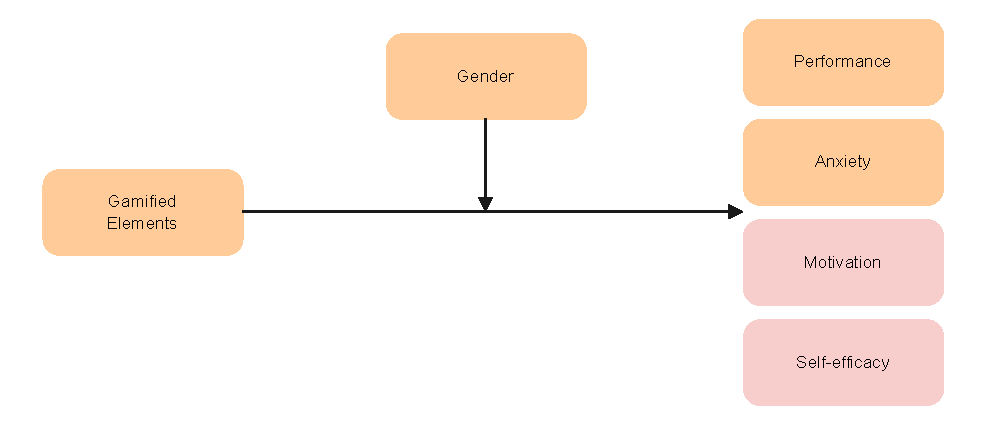
\includegraphics{img/Hypotheses}
    \caption{This diagram illustrates the impact of gamified elements (independent variable) on performance and anxiety (dependent variables), mediated by gender (mediating variable).}
    \label{fig:figureHypotheses}
\end{figure} The hypotheses we want to investigate in this work are:
\begin{itemize}
    \item[H1] Males and females differ in their cognitive and affective states.
    \begin{APAitemize}
        \item[a)] Male performance is better compared to female.
        \item[b)] Male and female students differ regarding their anxiety levels.
    \end{APAitemize}
    \item[H2] Different gamified elements have a varying impact on the cognitive and affective states.
    \begin{APAitemize}
        \item[a)] Gamified elements impact performance differently.
        \item[b)] Different gamified elements impact anxiety levels differently.
    \end{APAitemize}
    \item[H3] Different gamified elements differently impact the cognitive and affective states of males and females.
    \begin{APAitemize}
        \item[a)] The influence of different gamified elements on performance differs between males and females.
        \item[b)] The influence of different gamified elements on anxiety levels differs between males and females.
    \end{APAitemize}
\end{itemize}